\graphicspath{{literature_review/fig/}}

\chapter{Literature Review}
\section{Biosensors}
Biosensors are employed in applications such as disease monitoring, drug discovery, and detection of pollutants, disease-causing micro-organisms and markers that are indicators of a disease in bodily fluids (blood, urine, saliva, sweat).\cite{bhallaIntroductionBiosensors2016} 
\subsection{Background on Biomarkers}
A biomarker is an objective measure that that gives an indication of the biological processes happening inside the body at a given moment.\cite{BiomarkersNationalInstitute} They are physical substances found in the body that can be measured. The concentration of biomarkers differs between healthy individuals and individuals with diseases, thereby aiding in diagnosis and monitoring of diseases.\cite{rosenzweigWhatArePancreatic2018} Some biomarkers are easy to measure (such as blood pressure, body weight, etc.) while others require tests of blood, urine or tissue samples.\cite{BiomarkersNationalInstitute} 

This project will focus on the detection of biomarkers found in blood samples such as the CA-19 biomarker used for pancreatic cancer detection. Note: Verduidelik bietjie oor CA-19. The concentration of these biomarkers in blood can give an indication of the presence and progression of a variety of diseases, including many types of cancer.\cite{ribeiroApplicationsElectrochemicalImpedance2024}

\subsection{Types of Biosensors}
A biosensor consists of an analyte, a bioreceptor and a transducer mechanism combined with the electronics needed to process the signal.\cite{bhallaIntroductionBiosensors2016} The analyte is the substance of interest (such as biomarkers) that needs detection. Bioreceptors are molecules such as enzymes, cells, DNA or antibodies that specifically recognise the analyte. These bioreceptors produce a signal (in the form of light, heat, pH, charge or mass change, etc.) when they interact with the analyte.\cite{bhallaIntroductionBiosensors2016} Antibody based biosensors are the type of biosensor that will be used to detect biomarkers in this project.

Antibodies are produced by vertebrates as part of their immune response to foreign organisms or substances (called antigens). They are the most common biorecognition element used in biosensors.\cite{zengRecombinantAntibodiesTheir2012} Antibodies are Y-shaped cells that can be divided into two distinct regions. The top of the Y is variable and binds to a specific antigen depending on the amino acids present in this region. The amino acids present in the constant region (the bottom of the Y) is similar between different classes of antibodies (within the same species of animal).\cite{zengRecombinantAntibodiesTheir2012} This constant region binds to the substrate of the biosensor during immobilization, leaving the variable region free to bind with antigens.\cite{suedaAntibodyImmobilizationImmunosensing2022a}
\begin{figure}[ht]
    \centering
    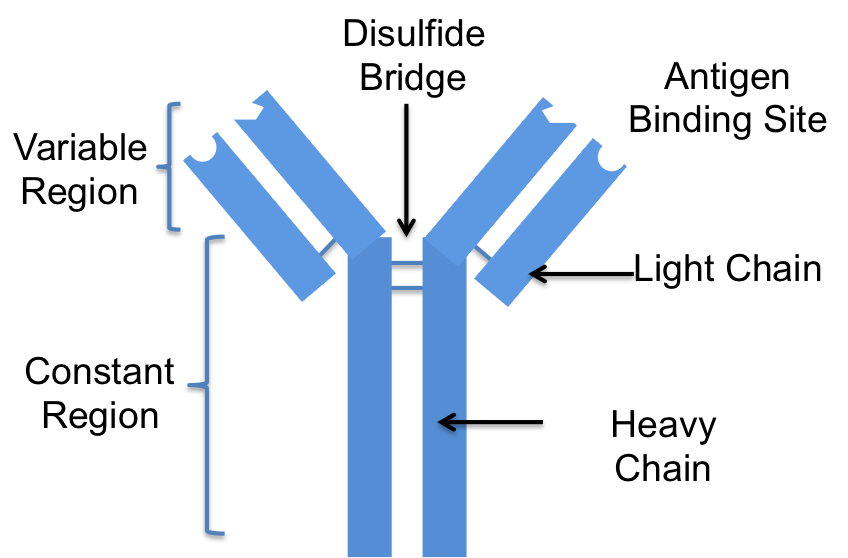
\includegraphics[width=0.7\textwidth]{antibody.png}
    \caption{Example figure inserted using a LaTeX Workshop snippet.}
    \label{fig:antibody}
\end{figure}

\subsection{Transducer Mechanisms}
The number of biological binding events indicates the concentration of the analyte in the sample. These binding events change the electrical properties of the biosensor, specifically the complex impedance. Thus, in order to convert the bio-recognition event into a measurable signal, a transducer mechanism is needed\cite{bhallaIntroductionBiosensors2016}. There are various types of transducer mechanisms that can be used in biosensors, including optical, piezoelectric and electrochemical transducers. 
EIS
Noem fardaic vs Capacitive sensors. Ons is capacitive.

\section{Signal Processing}
\subsection{Analogue Electronics}
\subsection{Digital Processing}
\subsection{Calculating Impedance}
\subsection{Extrapolating from Impedance to Concentration}

\section{Interface}
\subsection{ESP32}
% \subsection{WebBLE}

\section{Related Works}

\label{chap:literature_review}